\section{Training}

\subsection{Multi-Task Joint Training Strategy}

To bridge the modality gap and align continuous audio encoder representations with the semantic space of the LLM decoder, we adopted a unified multi-task joint training strategy. Rather than treating audio-language alignment as an isolated pre-training phase, the model was trained simultaneously on automatic speech recognition (ASR), speech emotion recognition (SER), and descriptive emotion analysis (DEA). SER and DEA serve as the primary emotion-centric objectives, while ASR acts as an auxiliary grounding task that connects acoustic signals with linguistic content. This design strengthens the model's ability to reason over both what is said and how it is spoken \cite{Qwen-Audio, SALMONN}.

To ensure robust multilingual generalization without overwhelming the emotion-centric tasks, we adopted a diverse sampling strategy for the auxiliary ASR data. Rather than using the full volume of available corpora, we aggregated representative subsets from a broad set of open-source datasets. The Mandarin subset comprised WenetSpeech \cite{WenetSpeech} and AISHELL \cite{AIShell}. The English subset included GigaSpeech \cite{GigaSpeech} and the LibriSpeech corpus \cite{LibriSpeech}. Additionally, we incorporated the proprietary Amphion multilingual in-house dataset. This curated mixture increased acoustic and semantic diversity while maintaining task balance, covering speech across varied lengths, domains, and recording conditions.

To improve robustness against real-world acoustic degradation and environmental domain shifts, we implemented an on-the-fly data augmentation pipeline. First, we applied additive background noise with a probability of $p{=}0.5$ at a signal-to-noise ratio (SNR) uniformly sampled between 10\,dB and 30\,dB. The noise profiles were sourced from the DNS Challenge~4 dataset (encompassing AudioSet \cite{AudioSet} and Freesound \cite{Freesound} clips) and the MUSAN corpus \cite{Musan}. This provided a rich mixture of background music, generic environmental noise, and overlapping background speech. Subsequently, we convolved the audio utterances with diverse room impulse responses (RIRs), encompassing both real and synthetically simulated acoustic environments.

During this joint training stage, we used low-rank adaptation (LoRA) \cite{LoRA} for efficient adaptation of the LLM backbone. LoRA modules were injected into all linear projection layers within the attention mechanisms and feed-forward networks, while the audio encoder remained frozen as shown in \Cref{fig:model_arch}. The LoRA configuration used a rank of $r{=}64$, a scaling factor of $\alpha{=}16$, and a dropout rate of $0.05$.

% TODO: add hardware, optimizer (AdamW betas/weight decay), LR schedule, batch size, total steps
% (required by reproducibility.mdc §1 and evaluation-metrics.mdc §3.1)


\subsection{Post-Training Alignment}

Direct Preference Optimization (DPO) \cite{DPO} has emerged as an effective technique for aligning model outputs with human judgments by contrasting preferred and rejected responses, with recent work demonstrating its utility in emotion-aware speech generation \cite{gao2024emodpo}. Achieving meaningful alignment for emotion understanding, however, requires preference data drawn from genuinely difficult in-the-wild samples---the kind that arise when models face acoustic degradation, sarcasm, or dynamic tonal shifts---rather than from scripted or easily resolved examples. The shift in the field's training data from small acted corpora such as IEMOCAP \cite{IEMOCAP} toward large naturalistic datasets such as MSP-Podcast \cite{MSP-Podcast} reflects the same recognition: real-world acoustic variability is a prerequisite for robust affective reasoning.

Building on these insights, we implemented a targeted post-training alignment phase using Emotional Direct Preference Optimization (Emotional DPO), an on-policy DPO variant focused on the DEA task. While supervised fine-tuning established strong generalized capabilities, Emotional DPO was used to further refine the model's descriptive emotion narratives on complex and ambiguous acoustic edge cases that are especially important for real-world emotion understanding.

To construct the DEA preference dataset, we leveraged the difficult samples previously isolated during our human-in-the-loop adjudication phase---specifically, instances involving intense acoustic degradation, subtle sarcasm, or dynamic multi-tonal shifts where standard models frequently misalign. For each identified hard case, we generated contrastive DEA response pairs: the human-corrected, expert-verified descriptive annotation served as the ``chosen'' (preferred) response, while the model's current on-policy DEA generation (or the initially flagged hallucination) served as the ``rejected'' (dispreferred) response. \Cref{fig:dpo_example} illustrates one such preference pair.

% TODO: convert to TikZ figure — domain-constraints.mdc §9
\begin{figure}[t]
\centering
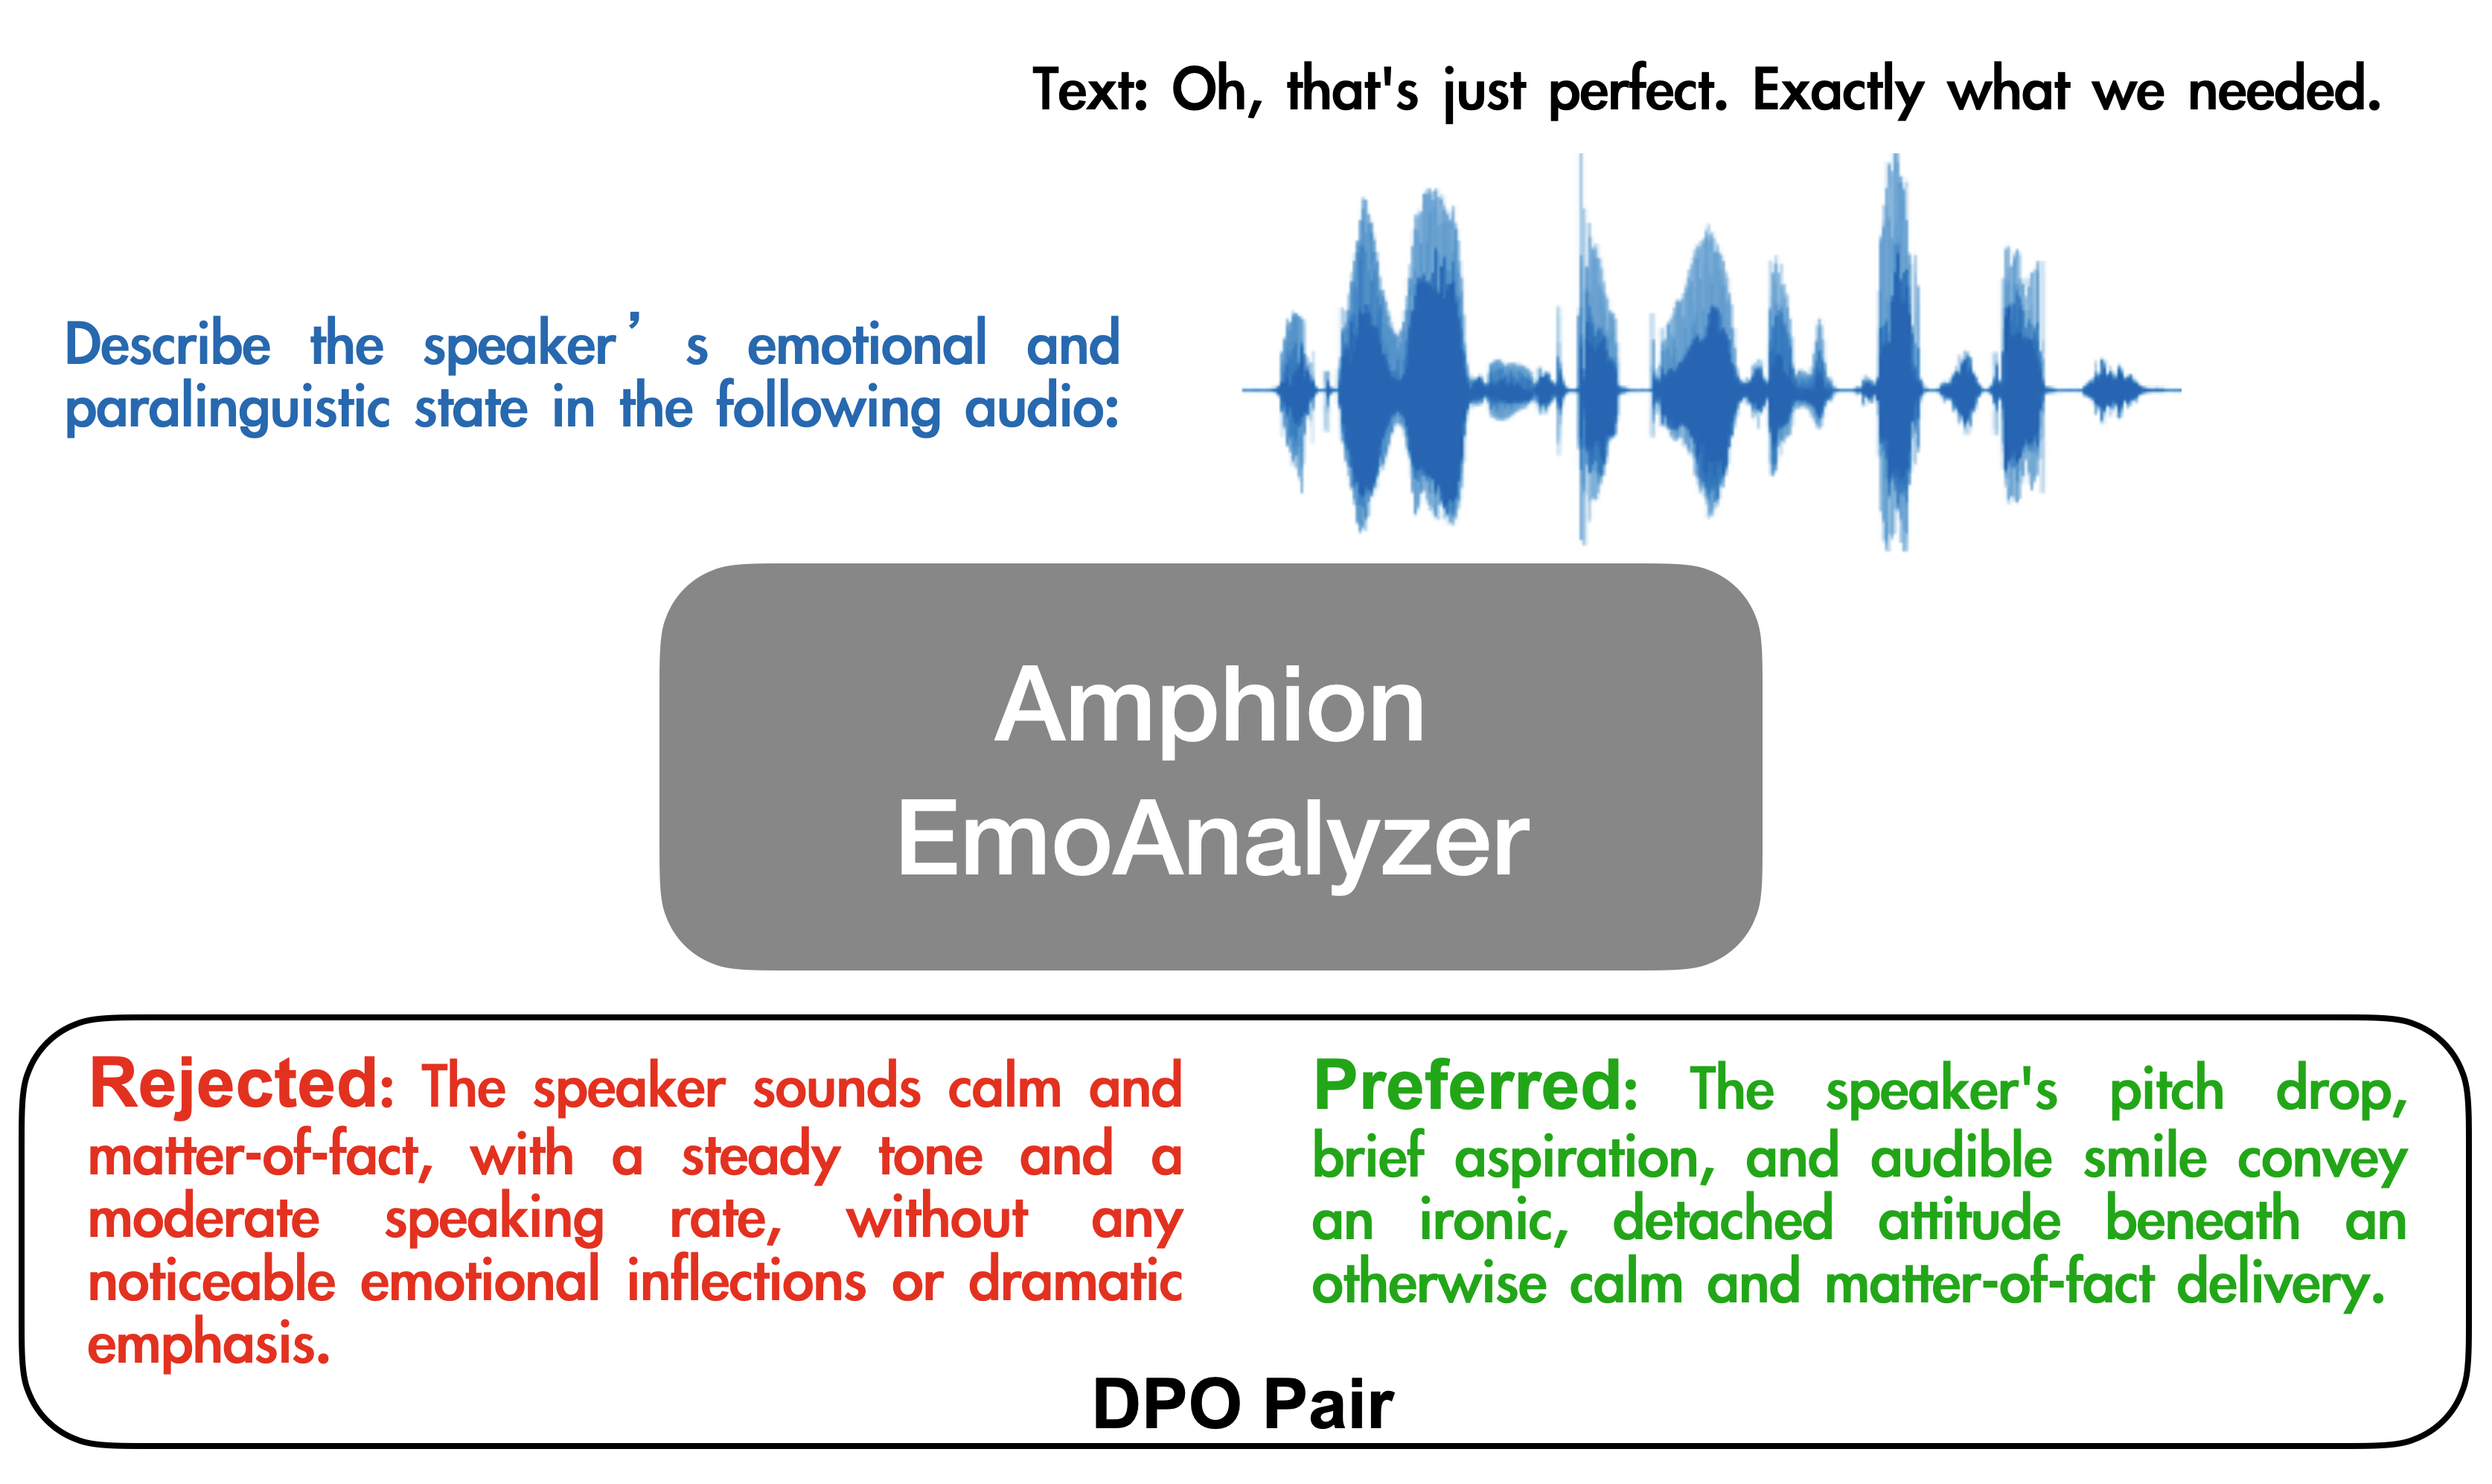
\includegraphics[width=0.75\linewidth]{images/dpo_example.png}
\caption{Example of DEA-focused Emotional DPO preference construction. Given a hard emotional utterance, the model-generated DEA response may miss subtle paralinguistic cues, while the human-corrected preferred response provides a more grounded emotional description for alignment.}
\label{fig:dpo_example}
\end{figure}

By applying Emotional DPO on these curated contrastive DEA pairs, we optimized the policy to penalize superficial acoustic reasoning and reward stronger paralinguistic alignment in natural-language emotion descriptions. This approach significantly mitigated edge-case hallucinations in DEA outputs, while also improving categorical SER predictions through more grounded shared emotion representations.

% TODO: add KL coefficient / beta, DPO preference dataset size
% (required by reproducibility.mdc §1 and evaluation-metrics.mdc §3.1)
